\section{Statistical uncertainties on data points}
\label{app:dataerrorbars}

Plots in this TN are produced with a symmetric vertical error bar on data points corresponding to the square root of the bin count. This approach is common in the field and it has the advantage of an immediate interpretation of the errors. However, given the low statistics regime of the analysis, it was suggested to use an asymmetric representation of the errors covering the 68\% confidence interval around the data observation. Our code supports this option as shown in Fig.~\ref{fig:dataerrs}. We are thus in the position to apply any centrally recommended option for the statistical uncertainty of the data, and will do so for the plots that will be made public. Note that the error bar on data points is used only for visualization and is not used for any rigorous statistical interpretation of the data.

\begin{figure}[H] 
\begin{center}
    \begin{subfigure}[b]{0.4\textwidth}
    \centering
    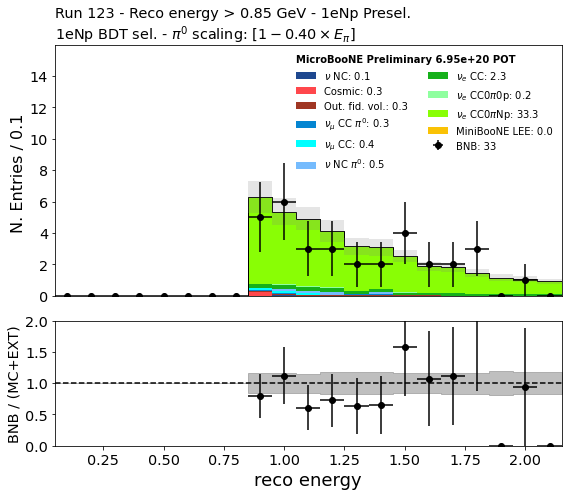
\includegraphics[width=1.00\textwidth]{Appendix/Figures/symm-sqrtN.png}
    %\caption{\label{fig:1e0p:dataMCRun1:shr_start_y} shr\_trk\_sce\_start\_y }
    \end{subfigure}
    \begin{subfigure}[b]{0.4\textwidth}
    \centering
    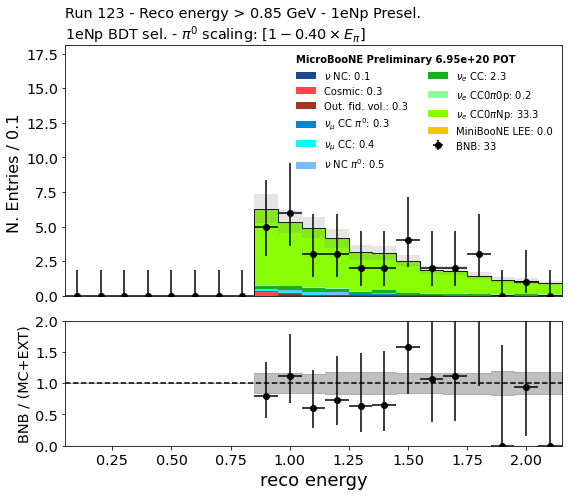
\includegraphics[width=1.00\textwidth]{Appendix/Figures/asymm-classical.png}
    %\caption{\label{fig:1e0p:dataMCRun1:shr_end_y} shr\_trk\_sce\_end\_y }
    \end{subfigure}
\caption{\label{fig:dataerrs} Reconstructed neutrino energy distribution in the \npsel high energy sideband with symmetric (left) and asymmetric (right) statistical error bars associated to data points.}
\end{center}
\end{figure}
